% Add a note about making connections to folks we don't explicitly connect you to, but don't lose track of hte plots we've already given you!
%%%%%
%%
%% This is intended as a nearly complete rules and scenario document
%% that you, the GM, change and complete for your game.  Various
%% comments suggest what parts can be removed or changed based on
%% common game variants.  For example, you will not need the rule for
%% player rooms if your gamespace is not open or otherwise doesn't
%% include living spaces.  Some possibly useful sentences/paragraphs
%% are simply commented out.
%%
%% Feel free to ignore these comments and just write what you want.
%%
%%
%%
%% These rules are merely an example ruleset.  Nothing in them is
%% sacred or even established by consensus.  They do not prescribe a
%% standard.  As a GM, you can change, remove, or rewrite whatever is
%% necessary to fit your game design.
%%
%% However, much of the material presented here, especially in the
%% Getting Started and Items Etc. sections, may be taken for granted
%% by many players.  This has two major implications:
%%
%% 1) Because of gradual shifts, longstanding biases, and first
%% impressions, different players (and GMs!) may have very different
%% assumptions about some details.  Do not brush off the sections that
%% "everyone knows."  Make sure everyone pays attention to the rules
%% as a whole.
%%
%% 2) If you have a clever idea to change some detail in the
%% fundamental parts of the rules, make sure to draw attention to it.
%% For example, if you modify the item bulkiness rules, don't just
%% gloss over your changes in the middle of a paragraph.
%%
%% You may want a section at the end as a reference to any fundamental
%% changes.  See "New Rule Summary" at the end.
%%
%%
%%
%% The martial combat system (and related health states and ranged
%% combat system) in this doc is known as "darkwater," named after The
%% Pirates of Darkwater, for which the first version was written.  It
%% is included as an example combat system.
%%
%%
%%
%% Basic guidelines for rules-writing:
%%
%% Use simple, concise, and precise language.  Avoid colloquialisms
%% and speech mannerisms.  Write in the second person.  Use the
%% imperative voice when possible.  Write like you are writing
%% directions.
%%
%% When you change contexts, like going from writing to the attacker
%% to writing to the defender, at least change paragraphs.
%%
%% When first introducing a major term and/or abbreviation, use bold
%% text.  Try to define terms before you use them.  Combined with
%% section/subsection/paragraph headings, this will make the rules
%% easier to skim for reference.  First establish context, then go
%% into detail.
%%
%% Be thorough, but do not ramble.  Try to make the spirit of the
%% rules clear in addition to the letter.  If the spirit is hard to
%% relay, then the rule may be too complicated.
%%
%%%%%

\documentclass[sheet]{GL2020}

\usepackage{graphicx}
\graphicspath{ {./images/} }
\usepackage{xcolor}
\usepackage{hyperref}
\usepackage{multicol}
\usepackage{ltablex}
\usepackage{tabularx}
\renewcommand{\tabularxcolumn}[1]{m{#1}}
\setlength{\columnsep}{1cm}

%% document-wide tweaks
\interlinepenalty10000
\setstretch{1}
\def\mytype{Rules and Scenario}
\lfoot{}\rfoot{}

\begin{document}

%% layout for cover page
\thispagestyle{empty}
\parskip0pt

%% title box
\begin{center}\LARGE\bf\begin{tabular}{|c|}
  \hline \gamename\\ \gamedate\\ Rules and Scenario\\ \hline
\end{tabular}\end{center}

\vfill\vfill

This game and all materials thereof are copyright 2021 by Acata Felton, Jeremy Cole, Kelsey Miranda, and Koh Henderson.\\

\vfill\vfill

\begin{center}\bf
  BROUGHT TO YOU BY THE LUMINARY ROLEPLAY SOCIETY
\end{center}

\vfill

\clearpage

%% layout for Table of Contents page
\thispagestyle{empty}
\tableofcontents

\clearpage

%% layout for main body of rules
\setcounter{page}{1}
\parskip5pt
\vfill
\section{Introduction}

The following are the rules for {\em\gamename}, a real-time, real-space, roleplaying game sponsored by the Luminary Roleplay Society.

\subsection{Expectations for Players}
You are responsible for knowing and following these rules. It is through the constraints created by these rules and other mechanics that interesting character to character interactions are made possible. Many of these rules are nigh-impossible for GMs to enforce, and rely upon the honor system. Do not cheat. Do not abuse loopholes. Play fair. To do otherwise will deprive both yourself and your fellow players out of the experience you signed up for.

The number of pages of reading for this game is between 30 and 40 pages for most characters. This is across all of the documents (including this rules document). Make sure you set aside enough time to prepare for game by familiarizing yourself with all of the documents. You do not need to memorize anything (except maybe your CR stat), but you should read everything in detail at least once, and know where to look up information. Print copies of everything will be provided at registration.

\subsection{GM Commitment}
The \textbf{gamemasters} (\textbf{GMs}) run the game. If you have any problems or questions concerning the game, contact a GM. Rulings the GMs make are final.  They may violate the letter of the rules to preserve the spirit.  The GMs promise to be as fair and reasonable as possible. Neither they nor these rules are perfect, so we ask for your understanding and flexibility.

\subsection{Disclaimers and Acknowledgments}
This game is a work of fiction. The attitude of the characters and the social milieu of the game world do not necessarily represent the opinions of the GMs, or of the player playing that character. While any work of fiction must draw some inspiration from real world situations, it is not intended to be a replication or direct allegory of any real world experience. We understand that the player experience is necessarily grounded in their own lived experiences in life, and have done our best to be mindful of the ways that game content can interact with that. Special thanks is due to <SENSITIVITY CONSULTANT(S) If they choose to be listed> for their time and effort to support this work. 

\subsection{Game Style}
This game is Secrets and Powers (S\&P) style (or ``Lit Form’’ if you are more familiar with that term), similar in style to  \emph{The Neptune Ball}. Game content is created by the GMs, and hooks are given to players to start various plots. Character goals may be mutually exclusive, leading to character vs. character conflict. Players will get the most out of the game by embracing their character, playing to discover the world created by the game writers, and reacting to new revelations from other PCs in character. Players may not come out of this game having accomplished everything their character wanted. 

While characters are often “playing to win”, players should look to the best stories. Embrace the most narratively impactful moment to have your character back down, admit a failure, spill a secret, or change their mind about something. You may find another character revealing your secret without any input on your part. This allows players to lean in to characters who want to keep a secret hidden.

This game also contains significant interactions between PCs and the environment. These interactions are regulated through predefined mechanics that allow players to interact with elements of the environment without waiting for a GM to narrate something or make a ruling. This generally leads to less sitting around waiting out of character, and more time playing and interacting in character. 

\subsubsection{Player Experience}
Players should expect to spend time before the game familiarizing themselves with game material, and preparing any costuming they choose. There is no need to connect with other players before the game - there will be time for that during workshops. During the game, players should plan to spend as much game time as they like in character, interacting with each other, and the world. Players should not expect to need to spend extensive periods of time out of character, negotiating things. Scenes can typically go wherever the characters take it, unless someone uses a safety mechanic (see below).


\section{Logistics}
\subsection{Basic Information}
\begin{itemize}
  \item \textbf{Dates and Times:} Players will be expected to be on site at the event location from 12 pm (noon) on Fri, Nov 12th - 5 pm on Sun, Nov 14th. Arriving late or leaving early requires special dispensation from the GMs. Please request any such arrangements well in advance.
  \item \textbf{Location:} YMCA Camp Jones Gulch, 11000 Pescadero Creek Rd, La Honda, CA 94020.
  \item Meeting Location: Dining Hall, side closest to ``South Tolowa Village''. Parking is available behind the Band Shell building. The event will begin with registration and lunch. See map below.
\end{itemize}

\begin{center}
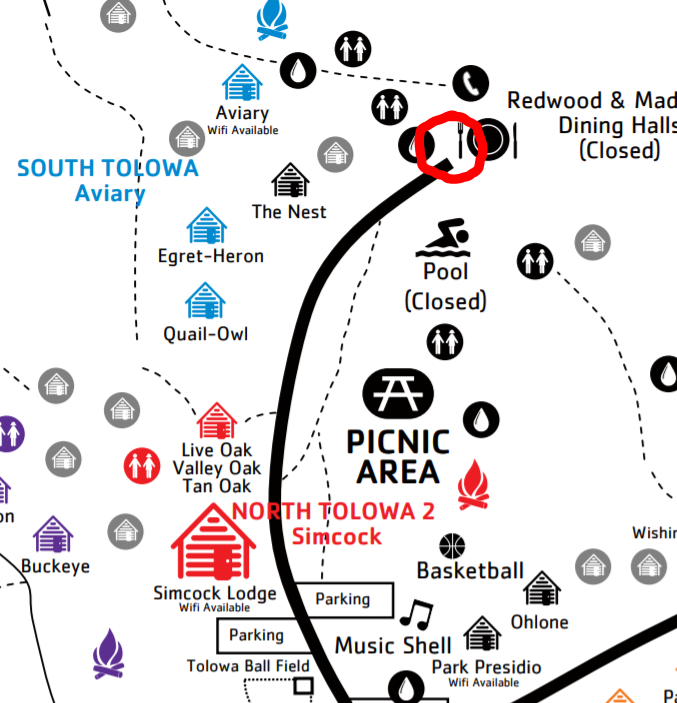
\includegraphics[scale=0.5]{CampMap}
\end{center}

\subsection{Game Areas}
The portion of the camp that we have reserved is primarily the ``South Tolowa Village’’ area. Most of the cabins in this area are game areas, along with Gyro Lodge (labeled as ``The Nest'' in the image above), the fire pit, and the deck of the dining hall nearest our camp. Game will take place both indoors and out. While we have also reserved the Band Shell for the duration of the weekend, we will be using it only for out of game activities due to its relative distance from the other game spaces.

Two cabins will remain entirely out of game: ``Banana Slug,’’ which will serve as the Out of Game Space from 10 am - 9 pm each day, and ``Aviary,’’ which will serve as the GM Headquarters. In the remaining cabins and lodge, the private rooms which sleep 1 person will also remain out of game throughout the event. All cabin spaces will be closed as game spaces when the first person staying there retires for the night (indicated by a sign on the door.). The fire pit, the deck of the dining hall, and the main portion of Gyro Lodge will remain open to \textbf{quiet} gameplay until midnight.

\section{Game Content}
As this game is a S\&P, the GM team can provide you with a lot of information about the premise and direction of game, as well as the types of personal plots and stories that are likely to show up.

\subsection{The Premise}
\emph{Welcome to the world of Cengea. The Gods have gifted the people with magic, but at a cost - the ravages of magical devastation roam across the land. Only a chosen few students can manipulate the path of these magical storms before their magic fades with age. Until recently, a treaty ensured a tenuous peace. The three nations agreed that the storm should hit each nation in turn, sharing the burden. Although the storms took their toll, no one nation suffered too greatly. That all changed when the treaty was broken and one nation was betrayed - and although architects and diplomats struggle to repair what was lost, their work won’t be completed by the next Time of Deciding.}

\emph{Our story begins at the center of the known world. Here at the \pSchool{}, students are trained in the rituals necessary to change the path of the Storm. Instructors maintain the veneer of impartiality - but in reality, the faculty is composed of the best operatives each nation has to offer, all vying for control of the magical disaster. But despite their efforts, no nation has the complete picture, and new interests conspire to change the fate of the world. Where the magic will ravage next - and what consequences it will have - are for you to decide.}

\subsection{Themes and Topics}
This game is set in a fantasy world with strong magical, and religious elements. Not all is well however, and the people in this world are facing many difficult choices. We ask that players prepare to engage with these themes, as they constitute much of the fabric of the world.

While having fun is a primary goal of many of our participants, it is important to recognize that some of the themes and topics addressed in the game are not light or fun. All of the characters are facing very serious moral and ethical choices that have real world analogies in the abstract, if not the specific. It is possible to both have fun at this game, and not dismiss the gravity of the decisions being made, and the consequences they will have.

\subsubsection{Magic and its Price}
Magic in this world is the source of almost everything. Food cannot be grown without magic, certainly not enough to feed the population. Ships cannot be built, certainly not well enough to withstand a sea serpent attack. Technology runs on magical energy, and cannot be made to function without it. There is no corner of life on \pEarth{} that is not dependent on magic. The characters in this game cannot conceive of a world without magic. It would be like the players living in a universe without gravity.

The Storms are also magical in origin and nature. Every three years, a magical storm brews over the lake where the \pSc{} is, and then whirls off to cut a swath of destruction across the continent. Until now, no one has been able to figure out how to stop this from happening. The best anyone could do was use the Ritual to direct the storm toward a particular country. This is not a trivial problem to be solved overnight - it has shaped the land, the lives, and the politics of \pEarth{} since magic began.

\subsubsection{Religion}
Religion is a big part of this world, and the lives of all of the characters. To help bring the world of \pEarth{} to life, we ask players to engage with the trappings of the religion, at least casually. As part of workshops, the players from each nation will create several common practices they share. The clerics of each religion will also pick and announce a time for a short religious ceremony of some kind (recommend no more than 15 minutes) during the weekend. If you miss it, it is reasonable to expect social consequences, even if you have a very good explanation.

This serves a few purposes. One, this is not a game of ``atheist superiority.’’ The Gods exist. They gave people magic. They appear to people, or speak through their Avatars frequently. It would take a lot to make someone a true atheist, or even agnostic in this world. The most lively areas of study all involve innovative magic use - there is no way to separate the intellectual from the magical from the religious in this world. This is an intentional part of the fiction of the world. Two, participating in shared rituals helps create a deep sense of connection and community between the characters, which is an experience we hope to foster for the players. Three, for those few characters that do reject part or all of the religion, the experience of trying to navigate a religious world can only happen if the rest of the players help create that world for them to navigate.

\subsubsection{Morality and Ethics}
On a national scale, morality is dictated by the religion, and governments endeavor to set rules and laws in place that reinforce this. On a personal level, many characters have opinions, not all of which align with the national and religious agenda. This game is absolutely meant to be a space where characters can engage in discussions about morality and ethics. However, we ask players to set aside some time to think seriously about the fact that your characters have grown up in this world, with very few dissenting voices. You should be prepared to argue for and support the status quo unless you have a specific reason outlined in your character sheet to question it.

We know that some of the morals that the fictional societies uphold are likely to be orthogonal, or even contradictory, to what some of our players believe in real life. We ask you to resist the urge to modify your character’s opinions to match your own too early in the weekend. This phenomenon is common in games ( sometimes called the “21st century morality problem”) and can very quickly cause tension and conflict to collapse. Many of these characters have hills they are willing to die on (sometimes literally), and the game will be more interesting if you are willing to stick to that until another character persuades you otherwise. 

\subsection{Content Warnings}
This game deals with a number of serious, and potentially activating topics. We have done our best to provide a list below of the most widely reaching content. Almost every character will bump up against these. Some characters will have large swaths of their play built around them. Players are asked to treat these topics with the gravity they deserve.

\subsubsection{War}
There is a war going on in the world of this game. It has been going on for almost 6 years. Many characters have been directly or indirectly involved; and everyone has been impacted in some way. War is not a conflict we introduce lightly. A lot of people end up dead, or mentally or physically disabled as a result of war, even in a fictionalized world. But much like in real life, many people are convinced that it is necessary, or that it is just, or that there is no way out that saves face (and that saving face is important.) While there is an opportunity in game for the characters present to try to forge a cease-fire or a peace treaty, the ultimate decision to ratify a treaty does not rest with the players. Instead, characters can submit correspondence to be sent to their respective governments (managed by the GMs), who will ultimately approve or reject proposals. This structure exists, not to take agency away from players, but to avoid trivializing the solution. 

\subsubsection{Nationalism and Jingoism}
Aside from the immediate effects of war, \pEarth{} is a continent at war. Nations have done everything they can to amp up national pride, and a sense of righteousness of their own cause. Leaders in every country are happy to villainize those from elsewhere, to create a boogeyman that keeps the fear and anger that started the war burning hot. The students are somewhat insulated from these effects inside the \pSchool{}, but the advisors should bring an extra-heavy dose of this into game.

\subsubsection{Religion and Spirituality}
We understand that not all of our players are religious or spiritual in their own lives, and that some folks may have trauma around organized religion (one of your GMs does). Being a part of this highly religious world may feel strange or uncomfortable, especially at first. We ask players to take particular care to avoid sharing a cavalier attitude toward religion and spirituality during and around this game, or to assume that ``everyone'' believes something or other out of character. \textbf{Players} should avoid proselytizing, whether about religion, spirituality, atheism, or other. (There isn't much proselytizing in character either; each nation is happy to have new people join their sect, but generally respect each character's choice of religion.) Let people have their own lives, do not assume that their character attitude reflect their player attitude, and do not offer unsolicited advice or opinions about religion or spirituality.

\subsubsection{Murder}
In the world of \pEarth{}, the Gods declared murder the ultimate crime, and enforce punishment themselves. The person who took another life loses their memories. Pretty much all memories, usually immediately, regardless of the circumstances. Some characters are interacting closely with plots that more directly address this, others are more removed, but it is a fact of this world. 

Even though character memory loss is a possibility, abelism is \textbf{not} part of this game. Characters can be suspicious of another character claiming not to remember things, but you should be careful about jumping to the conclusion that it is divine amnesia; plenty of people lie all the time about not remembering one thing or another for a variety of reasons. It is also important to distinguish that some \emph{players} may have difficulty remembering things. Be kind and patient with each other if someone asks for you to clarify or repeat something you said previously, or needs to refer to a game document.

If one character succeeds in killing another character during the game, that character will suffer memory loss starting immediately at the end of game. The reasons for this are explained in more detail below, in the section on combat, subsection ``Killing Blows and Character Death.’’

\subsubsection{Potential Apocalypse}
It may be possible, through certain character actions or inaction, to cause an apocalypse level event that will drastically change the course of \pEarth{}n history. No change so drastic can come without significant fallout among many inhabitants, and the worst parts of it are likely to fall on the most marginalized communities even if they are specifically prepared (for example: if they are instigating the change.) Any decision you make that drives toward something like this should be made bearing this weight in mind.

\subsubsection{Content Warnings impacting PART of game}
\begin{multicols}{2}
\begin{itemize}
  	\item Family issues. Some characters have difficult relationships with biological family members, including estrangement.
	\item Established Romance - some characters are in established romantic relationships; at the discretion of the players involved, these can be re-imagined as platonic life partnerships.
	\item Potential Relationships - some characters are interested in exploring new romantic or platonic relationships with other characters. None of the feelings are unrequited, but some characters may not realize yet that someone else is interested in a relationship with them.
	\item Polyamory - Some of the existing or potential relationships involve more than two consenting adults.
	\item Cheating or infidelity - some characters may not be honest in their relationships.
	\item Harm to animals - the Avatars of the Gods typically take the form of sentient animals. Some characters may wish to do harm to those specific animals due to their avatar nature.
\end{itemize}
\end{multicols}

\subsubsection{Content Warnings NOT in game}
Due to the game design, we can provide the following list of topics and tropes that will \textbf{not} be part of the game material, and shouldn’t come up during play. This is not a complete list, and if you have questions or want to check about a particular other topic, please reach out and ask.

\begin{multicols}{2}
\begin{itemize}
  	\item LGBTQIA+ Discrimination.
	\item Fatphobia / fat shaming.
	\item Sexism.
\item Unwanted sexual attention (harassment, assault, etc.)
	\item Ableism - no characters are written specifically as abled or disabled. We do require abled players who choose to portray a disabled one to clear it with us first, and do so respectfully.
	\item No characters are soldiers or police, but some characters have positions of authority over other characters.
	\item Medical procedures. All healing is abstracted, and is not meant to support extended graphic roleplay scenes around healing or other medical procedures.
	\item pregnancy or pregnancy loss.
	\item Sex - while this game has several established and potential romantic relationships, there is no sex mechanic, and players are asked to avoid emphasizing those aspects of the relationships.
	\item Substance abuse.
	\item Partner or child abuse.
	\item Pandemics
\end{itemize}
\end{multicols}

Once you get your character, please stay within the bounds outlined by that sheet and the game content in general. Do not invent edgelord backstory elements, or introduce new plot points. This is important for the integrity of the game. If you invent something new and abandon content written for the character, you leave the other characters involved in that content out in the cold. This is also crucial for the safety of your fellow players since they didn’t get a chance to opt into or out of the new content. If something isn’t working for you, get in touch with the GM team as soon as possible, and we’ll work together to find a solution.

\section{Safety}
This is only a game.  Everyone involved should act with courtesy, sportsmanship, patience, and taste.  The GMs may expel anyone they believe to be violating the spirit of the rules or the game.  Emotions may run high.  If you think things are crossing the line from game to reality too much, or if you are just getting too stressed, take a break. Always, play safely, then play to have fun. 

Real violence is unacceptable. Game action should cause no real-world damage, either to people or property.  If something dangerous is happening, call a halt.  Stay in control, use common sense, and do not endanger yourself or others.

Safety is a shared responsibility in the community, between all of the participants, players and GM alike. Only you can determine if you need to step away from a scene, plot, player, etc. Only you can say whether you need a temporary or a permanent solution. But we can all be aware of the ways that we interact with others, and be willing to adjust our behavior based on feedback for the safety and comfort of our fellow participants.

\subsection{Calibration}
\textbf{Players are more important than the game}. In this game, this adage must be applied preemptively, not just when someone gets activated in the middle of game. Secrets and Powers games are fragile. While they can survive a character not being present, the game is significantly the poorer for it. This is due to the design concept that any character the game could run without should either be cut before casting, or rewritten to be more integral. This makes it way less likely that a player will be bored or feel left out, but it does pose important considerations for safety.

Calibration is handled primarily through casting. Since players filled out the casting application for this game in January and February of 2020, we understand that some things have changed. Once you receive your character sheet, we ask you to read over it and let us know \textbf{as soon as possible} if there are aspects we need to change. Please don’t just change things on your own without talking to the GMs; we need to rebalance game around the changes.

\subsubsection{Self Care}
\textbf{Players are more important than the game}. Take some time in the days or weeks leading up to game to ask yourself what you need to take care of yourself. We want you to have the best chance of having an enjoyable experience at game, and contingencies in case that doesn’t happen. It is also a good idea to be prepared in case of drop or bleed afterwards. See the ``Deroll and Debrief section below for more information about these terms.:
\begin{itemize}
  \item Reflect on the game scenario and the listed content warnings (see above). If you have reasons to believe you’ll be activated by game content, start a conversation with the GMs so we can determine jointly if you’ll be able to avoid the activating content or not.
  \item Reflect on your mental, physical, and emotional reserves, and what actions you can take to prepare care for yourself before game to boost your resiliency (i.e.: making sure you get a full night's sleep before game). Consider what preparations you can make for self care after game to replenish (i.e.: ordering your favorite food for dinner, or bringing a stuffed animal for deroll and debrief). 
  \item Reflect on the safety mechanics (see below) for this game and how you can use them to protect yourself and create space to check in with yourself. If you need to, leave the game, temporarily or permanently. The door is always open, and if it’s what you need to take care of yourself, do it. But if a less nuclear safety mechanic feels accessible, we encourage you to try that one first.
\end{itemize}

\subsection{Safety Mechanics}
When in doubt, use the universal Out of Game symbol of: placing a fist on top of your head. Use this to go out of character and talk or do whatever you need to as players to re-establish a safe play space, or address an out of character situation. 

Your GMs will be available during game to assist and facilitate as well. During game on hours, we will either have someone available at GM Headquarters (Aviary), or leave a note with where to find us. We are not trained mediators, therapists, or counselors, but we care about you and want you to have a good time. We can help you come up with plans for self comforting, and when you are ready, help you decide if and how you want to re-engage with game.

The following safety mechanics will be used in ``\gamename{}’’. We will practice with these mechanics during workshops before game. Do not use the safety mechanics to escape from an angry mob out for your character’s blood. These are for player safety. Misuse of safety mechanics is unacceptable, and ignoring another player’s use of them will have disciplinary consequences.

\begin{tabularx}{\textwidth}{|>{\centering\arraybackslash} m{1.5cm} | >{\centering\arraybackslash} m{1.8cm} | >{\centering\arraybackslash} m{1.8cm} | >{\centering\arraybackslash}X |}
\hline 
 \textbf{Mechanic} & \textbf{How to Use} & \textbf{What happens next} \\
\hline
Out of Game Hand Signal & Make a fist with one hand. Place it on top of your head (visible from in front of and behind you) & You are now out of character (OOC). You may talk and act as your player. This is useful for many things including talking player to player about something that just happened that you need to adjust, stepping out to use the restroom, or because a mechanic told you to. If someone uses this around you, your character no longer sees theirs. You should ignore OOC players unless they address you directly and ask you to go OOC too to discuss something. If you need to have an extended conversation OOC, we encourage you to step away from ongoing game play so as not to disrupt it. \\
    \hline
``Okay Check In’’ & Make eye contact with the person you want to check with, and flash them the ``ok’’ symbol with your hand. They should respond with a ``thumbs up,’’ ``thumbs down,’’’ or ``thumbs sideways’’ & Use this mechanic to check in with someone who appears to be in distress (i.e.: crying), who’s demeanor has suddenly changed (i.e.: stopped talking and has a 50-yard stare), or you otherwise want to check in on whether the \textbf{player} under the character is doing okay. If you get a ``thumbs down’’ or ``thumbs sideways’’ response, try to pause game play and take a moment out of character to check in with the player. Encourage them to check in with themselves if they need to change anything about current play or the current environment. If you don’t feel able to check in with them at that time, find a GM or send them to GM HQ.\\
    \hline
``Brake’’ (from ``Cut and Brake’’, sometimes used as ``Largo’’) & Say ``Brake,’’ and put both hands out flat, at shoulder height, palms away from you. Push out into the air once or twice, like pushing the brakes of a car. & Use this to de-escalate the intensity of an interaction for a player’s safety or comfort. I.e.: Ask a player to speak more quietly, even though their character is still yelling, or take a few steps back, even if their character is still physically blocking yours in. This is not a negotiation - the person being asked to ``brake'' should immediately comply for the comfort and safety of their fellow players. \\
    \hline
``Game Halt’’ & Say ``Game Halt’’ in a loud enough voice for people right around the corner to hear you, but not so loud as to shout. End the halt once the issue is resolved by saying “3, 2, 1, Game On” &  Used to halt game play in a whole area, either for safety or a mechanic. This call should be used to halt game play to sort out a safety issue such as a player being too activated to continue at the moment, or in need of a longer player to player discussion for which ``brake’’ is insufficient, and everyone in the scene needs to be involved. This call should also be used for physical danger, for example: repositioning players so no one is at risk of falling down a cliff. This call is also used by some mechanics to pause the game to fetch a GM for something. \\
    \hline
``Badge Off’’ & At a time when you are not in the middle of a game action, simply take your badge off & Use this to indicate that you are exiting game for the night, or need to take an extended break from game (longer that would be comfortable to maintain the Out of Game Hand Signal). If you are going``Badge Off’’ for a game related reason, feel free to come find a GM if we can be of any help. Players should assume that another player without their badge is out of character for an extended period. You may take no game actions toward someone who isn’t wearing their character badge. If you are looking for their character, assume they cannot be found. \\
    \hline
``Open Door’’ & Physically leave the game space. & If you need to leave the game and not return, either for self care or emergency reasons, please do so. PLEASE, let a GM know so we don't start a search and rescue operation assuming you are lost in the mountains somewhere. \\
    \hline
 \end{tabularx}

\section{Out of Game Programming Events}
This weekend LARP, ``\gamename{}’’, has a number of out of character activities scheduled before, during, and after the game. These events are designed to help players enter and exit game play safely, and foster a sense of community. They also serve for GMs to reiterate rules and expectations, and for everyone to ask questions. While only the pre-game workshops are strictly mandatory, players are strongly encouraged to come to the optional activities as well. Since post game activities affect when carpools can leave, players should plan to be on site until 5 pm on Sunday, even if they personally wish to opt out of post game workshops.

\subsection{Pre-Game Workshops}
There will be three mandatory pre-game workshops on Friday afternoon. These workshops are designed to help players get into character, create shared cultural touchpoints, and foster trust among players. We have players coming from all over, many of whom have not played with each other before. These workshops should help create a space where players feel safe enough to play deep and intense character relationships if they want.

\subsubsection{Workshop 1}
For workshop 1, players will be split up by home nation. In this workshop we will introduce players and characters, and then spend some time creating cultural touchstones. We will also take some time to reflect on the impact that the war has had on the nation, and on the characters.

\subsubsection{Workshop 2}
For workshop 2, players will be split up by cohort (student, teacher, advisor). In this workshop we will introduce players and characters again, and then spend some time creating cultural touchstones. We will also take some time to reflect on the Time of Deciding, and the role each cohort plays in it.

\subsubsection{Workshop 3}
For workshop 3, players will be split up by the GMs in a mix across nation and cohort. In this workshop we will introduce players and characters one last time. We will talk about safety in a broad sense, and then review and practice the safety mechanics for this game in specific. We will also take some time to reflect on how magic is integral in these character’s lives and the world.

\subsection{Game Rebalancing}
This \textbf{optional} program on Saturday afternoon will be an opportunity for players to evaluate their play experience, and refocus if they wish. We will take some time to introspect on the play experience so far, and identify if there are things you wish to change about how you approach play, either internally, or interpersonally. We will close the activity by connecting players who feel overly busy, and those who feel bored or left out. These connections will have the opportunity to discuss player to player about how to bring characters into plots and share story. These conversations can continue into Dinner, which is \textbf{mandatorily} OOC.

\subsection{Post Game Workshops}
Formal deroll and debrief are optional, but highly encouraged activities after the game ends. If players prefer, they may opt out of the formal versions and take time on their own to reflect on their experience, but players are still expected to remain on site until 5 pm unless arrangements are made ahead of time. These activities help with\textbf{bleed}: character feelings affecting player experiences, in this case after the game (i.e.: a player is short with someone at work after an intense weekend game). These activities also help with \textbf{drop}: players feeling low emotions after interacting closely with people for several days and then going their separate ways.

\subsubsection{Deroll}
A formal Deroll will happen first. Players will have the opportunity to reflect either in a group, or individually on the experience of the weekend. We will take time to intentionally separate player from character, and provide opportunities for closure. This helps soften the transition from the liminal space of game back to our real world lives.

\subsubsection{Debrief} 
Debrief will follow Deroll. Debrief is an opportunity to learn the immediate post game consequences of character actions in game. Everyone will get a chance to share a little about who their character was and what they were trying to accomplish this weekend. This is a great opportunity to learn about the other stories being told over the weekend.



\subsubsection{Goodbyes}
This activity will be unstructured time after the close of formal programming for players to say goodbye. You’ll be able to hang out, tell war stories, ask each other and the GMs questions, etc. We’ll be sending everyone home at 5 pm.

\vfill

\clearpage
\section{Getting Started}

%% Character packets come first, since they are the tangible things handed to players.  Also a convenient place to define Player Character.
\subsection{Character Packets}

Your character packet is a big manila envelope.  It contains your role: who you are, what you're trying to accomplish; everything about your part as a {\bf player-character} ({\bf PC}) in the game.  Read all the contents and generally keep them with you during the game.  If you are missing something or find something which doesn't seem to belong to you, tell one of the GMs.  Character packets are confidential.  Game materials which cannot be given to other players are marked ``Not Transferable,'' whereas things which can be given to others are marked ``Freely Transferable'' or ``Game Item.''

Your Character Packet would normally contain:
%% other things your game uses, like money, should be described below

%% no character names on badges, yes to character descriptions
\paragraph{Name-Badge:} A name-badge with your character name, player name, character description, and {\bf badge number} on it shows that you are in the game; wear it visibly while you are playing.  It represents your character's body in-game.  Badge numbers are not in-game information. See the \emph{Character Bodies} and \emph{Badge Numbers} sections for more details.

\paragraph{Character Sheet:} Your character sheet describes who you are and what you are up to.  It contains a list of everything else that should be in your character packet.  Do not show or read your character sheet to other players.

\paragraph{Bluesheets:} A bluesheet describes information common to members of a group.  When in conflict, character sheet information overrides bluesheet information.  Do not show or read a bluesheet to other players.

\paragraph{Greensheets:} A greensheet describes and expands abilities, mechanics, or in-game knowledge.  Do not show or read a greensheet to other players.

\paragraph{Stat Card:} Your stat card lists your statistics, and is printed on pink or salmon colored paper.  You might not know what all of your stats mean.  Do not show your stats to others.  The reverse side is a {\bf death report}; fill it out and give it to the GMs if your character dies.

\paragraph{Ability Cards:} An ability card explains a special ability your character has,and is printed on yellow paper.  The front side (says ``Ability effect’’) describes the effects; show it to players when you use the ability.  The reverse is the rules of use and must not be shown to other players.

\paragraph{Memory/Event Packets:} A memory packet is an envelope or stapled piece of paper with a {\bf trigger} which describes when to open and read it.  If the trigger is a number, open the packet when you see something with that number.  If it's a quoted phrase, open when you hear or read it in-game.  If it's a symbol, open when instructed.  Do not take game action based on an unopened trigger.  Do not show or read a memory packet to other players.

\paragraph{Research Notebooks:} A research notebook is a little  booklet of pages folded over and stapled shut. These packets guide you through creating or researching something taking many steps, in which the full process that will be required is not known at the start. \textbf{You should open the first page when game starts}. Each page will describe information you learn, and tell you what action to take next. When you complete the requested action, you may open the next page. Do not show or read a research notebook to other players. 

\emph{Exception:} Some research notebooks will list other characters as having the same notebook. In these cases, if the \textbf{characters} elect to share information, plates may open pages to match.. I.e.: If player 1 has opened page 3, but player 2 has not, after conferring in character and agreeing to share information, player 2 may open pages up to and including page 3.

\paragraph{Items:} In-game items may be transferred from character to character, and should be marked as such.  See the \emph{Items Etc.} section for more details.


\clearpage
%% Some Assassin Game fundamentals
\subsection{Reality and Game Reality}

There is a big difference between reality and game reality.  Players must treat each other with courtesy and explain to each other what their characters perceive in confusing situations; e.g.\ ``My character's hands are covered in blood,'' an {\bf out-of-game} statement.  Characters are under no such restrictions, and may do what it takes to further their goals; e.g.\ ``Uh, hi Bob. Just got back from the butcher shop,'' an {\bf in-game} statement.

{\bf Metagaming} is inferring in-game knowledge that is inappropriate for your character from out-of-game information.  Do your best to not metagame and especially to prevent the risk of metagaming. Don’t eavesdrop on conversations when your character is not there. Do not read other player’s game documents, even if you both \emph{think} you have the same document because it is named the same. If you do come across information as a player that your character wouldn’t have access to, do your best to pretend you don’t (``firewalling’’), so it doesn’t influence your character decisions.

While some players may be more familiar with games with higher levels of transparency, not every player enjoys having to firewall a lot of information. Please do not volunteer information to another player that their character might not have. If necessary for safety, players may discuss secret character information ahead of time, but we generally find that this is necessary less frequently than you might think. Trust your fellow players to enjoy unexpected twists in the story as new information is revealed to players and characters simultaneously.

\paragraph{Not-Here:} Some mechanics may instruct you to go ``Not-Here.’’ You go not-here by turning your name-badge around so the ``I'm Not Here'' side is showing. Putting a hand on your head, visible from a distance, helps if you're near other players. When you are not-here, your character is not there.  Your character cannot see, hear, or remember any game actions or information you (the player) happen to encounter.  Avoid other characters, common game
areas, game signs, or any sort of game interaction. Going ``Not-Here’’ is a game mechanic. Doing so in front of other characters represents something like suddenly becoming invisible, and is distinct from the safety mechanics described above.

\paragraph{Non-Players:} Use tact and common sense when dealing with non-players ({\bf NPs}).  Many NPs prefer to sleep, study, or work undisturbed. Camp staff have their own lives, and other groups at the camp have their own events to attend. NPs may not knowingly affect the game. They and their rooms may not be used to hold items or information. Do not use the presence of NPs to hide from rampaging mobs that want your blood.

Avoid conspicuous or threatening game actions in front of NPs. Please keep conversations about murdering another character and other potentially activating topics out of earshot of NPs. Do \textbf{NOT} shout ``fire’’ unless there is a real life, actual fire.If there is an in-game fire, you may use stage whispers. If, despite your most valiant efforts, some NPs do get upset, call the GMs who will help calm them down.

If you are about to take an action that would likely upset a nearby NP, you may call a game-halt and relocate the scene. This is considered an out-of-game issue.

\paragraph{Out of Game Spaces:} Some of the spaces at the camp are ``in game’’ and some are ``out of game.’’ Players may spend time out of character in any of the out of game spaces in safety. Do not take game actions in out of game spaces, store in game items in these out of game spaces, or camp the entrance to an out of game space to ambush someone returning to game.

Players may rest or sleep whenever they choose. To preserve this for players, characters cannot be woken up or attacked while they are sleeping or resting. This is an out of character issue. Do not use this as a way to hide from angry mobs out for your character’s blood.

\paragraph{Observers:} An observer is someone not playing the game who has agreed to watch.  They generally wear an observer headband or an observer name-badge.  Observers have traditionally been called ``ghosts.''  They should stay out of the way; you can always ask an observer to leave.  If a friend who is not playing wants to observe game, send them to the GMs.

\clearpage
\paragraph{Mechanics:} Many actions your character can take, such as walking, talking, and general interaction with other characters, are represented by you doing them.  Others, like combat, are performed via abstract mechanics, which are described in ability cards, greensheets, and rules.  The abstract information for mechanics (like badge numbers) may not be discussed in-game.  If you want to do something special for which there is no mechanic, ask a GM.

Become familiar with your mechanics before game starts, especially those which occur under time-pressure (like combat).  Game action will not stop for memory packets, greensheets, or such.

A \textbf{kludge} (and derivative forms like ``kludge-ite'') is something impervious to logic and cleverness, usually for game-balance.  You can't affect a kludge without a specified mechanic, even if common sense tells you that in real life you could find a work-around.

Do not invent items or solutions to a problem that already has a mechanic. This is a kludge for game balance. If a door says it needs a key to open, you cannot declare that you beat the door down, nor can you claim to have the key if you don't actually have the key item (use item numbers to verify if you have the correct item. More about item numbers below).  If there is no mechanic, plots should be resolved via \textbf{in character} discussion (aka: roleplaying). If you aren’t sure, you can always check with a GM. 

{\bf Zone of Control} ({\bf ZoC}) is a rough distance measurement. You are within ZoC of someone if your outstretched fingers can touch their outstretched fingers.  Double-ZoC is twice this distance, triple-ZoC is three times, etc. You should not run or otherwise force your way into or through someone else's ZoC, and you should not make physical contact with another player without permission.


{\bf Headbands} represent obvious visual effects; wear them visibly on your head. If you see a headband and don't know what it represents, ask. If you are wearing a headband, tell people what their characters see.

An {\bf interruptible} mechanic has some duration, and may involve continuous roleplaying.  It is stopped if you are attacked or if someone within ZoC says {\bf ``I stop you''} or an equivalent phrase. Some mechanics may be easier or harder to interrupt.

A {\bf n-count} is an interruptible mechanic with a repeated, counted incant (``I pour a drink one, I pour a drink two, I pour a drink three'').  Speak clearly; each count must take at least a full second. Each n-count will specify the number, e.g.\ a 3-count.

\subsection{Basic Strategy}

Make sure you understand the rules.  If you are completely confused, get a GM who will try to help you out.  Make sure you know enough about your character to role-play him or her when you start talking to other people.  Read through your entire packet a couple of times, and skim through it again right before game starts.  If you don't know something about your character, ask a GM.

As a character, your first priority should be to open lines of communication.  Contact people, show up at meetings, and chat.  Try to be easy to get in touch with.  Ask people questions on relevant subjects.  They may lie, but you will probably find something out. There are no guarantees that you can trust anyone, but since cooperation is the key to accomplishing things, you will be forced to trust people anyway.  The most trustworthy people are probably those who need you.

\clearpage
\section{Items Etc.}

Many in-game items are represented by little white cards with a number and description.  Item cards may be shown to others, passed around, stolen, etc.  The {\bf item number} on the card is not in-game information and may not be discussed.  

Some mechanics in game may involve making item cards. Such items should be clearly marked as ``in game'' and treated as such.

Use common sense.  You can't carry a hundred rocks in your pocket, fold a sword in half, or hide a life-sized statue in a fire hose.  You can't stop a bullet with a set of blueprints or rip apart a metal safe with your bare hands.  Even if your bag can carry a shovel in it, the shovel noticeably sticks out (``you see a shovel sticking out of my bag'').

\paragraph{Written Information:} If you write in-game information down on a piece of paper, that paper is now an in-game item and must be clearly marked as such.  Don't write in-game information on out-of-game documents (character sheet, etc.).  Don't write out-of-game information (like memory packet triggers) on in-game documents. Paper and writing implements will be available at GM headquarters.

\paragraph{Envelopes:} Some items and locations may have an attached envelope (or just be a labeled packet or folded paper).  The envelope may include directions for when to open these (``open packet if you press the big red button'' or ``open packet if you eat this''); otherwise you may only open them if instructed.  Close them when you are done.  Open and close packets gently.

\paragraph{Signs:} Some locations and other game materials are represented by signs or packets posted throughout game area.  You may read any signs and must follow any rules printed on them.  If a sign or packet doesn't have some sort of in-game description (it only has out-of-game mechanics information, like a number or just a colored dot), then your character doesn't even see it or know that anything unusual is there.

\paragraph{Bulkiness:} A bulky item is too big or heavy to be carried or concealed freely.  Bulkiness is measured in {\bf hands} or {\bf dots} (how many hands it takes to carry it).  If you are carrying a bulky item, make it clear to onlookers (hold the card).  A hand carrying a bulky object may do nothing else.  With one hand less than required, you may drag a bulky item at a slow pace.

\paragraph{Props:} Some items may have props (physical representations or \textbf{physreps}) associated with them.  The card and physrep should be kept together.  \textbf{If they are separated, the card is the real item}. Prop items are as bulky as the physrep.  They can be carried in bags that can hold them, on straps that are attached to them, etc. If you bring your own prop to represent an item, you \textbf{must} attach the item card and display it prominently.

\paragraph{Character Bodies:} A body is {\bf three hands bulky} and usually represented by a name-badge.  It must be willing or unable to resist for you to carry it.  Carry the badge conspicuously.  Onlookers can't tell if it's dead without close examination, unless it would be
obvious (like headless). If you are carrying a PC, and that player is available, they should walk along with you. Please do not actually attempt to physically carry another PC.

\paragraph{Unstashable Items:} Unstashable items can't be hidden or left behind.  They look too important, valuable, or interesting; NPCs will not let them stay there.  These include any item that has a physrep. This is a kludge.  If you're not leaving an unstashable item in another PC's care, and you want to leave it behind, give it to a GM or observer.  You may leave it in plain sight in a public area if there are other PCs around.

\clearpage
\subsection{Searching, Stashing, and Stealing}

\paragraph{Places:} To search a place, search it.  Normal items can be stashed in any reasonable, legal place.  Don't put items behind locked doors, inside ceilings, in construction sites, or in hacking locations; consequently, don't go rummaging through such places for game items.  Don't stash or search in places that are not in-game; see the \emph{Game Areas} section for more information.

\paragraph{Doors and Locks:} Some doors or items in game are \emph{locked}. You may not open them or get past them unless you fit the requirements listed, or have some other method of opening locks. Closing such an item or door locks it again.

\paragraph{People:} All searches of characters or their belongings are conducted via player dialogue.  Someone must be willing or unable to resist for you to search them.  You need at least one free hand to search someone.  Searching is interruptible (see above).

You can perform a {\bf pat-down search}, which will only reveal the presence of weapons.  This takes as much time as it takes your victim to tell you what you find.  If you're the victim, do this at a reasonable pace.

A {\bf total search} is an invasive, complete search of a character's clothing.  This reveals all in-game items, and takes as long as your victim spends handing over possessions.  If you're the victim, hand over items at a reasonable pace.

\paragraph{Bags:} To search a bag in someone's possession, say ``I search your bag.''  This proceeds just as a total search.  To search an unattended bag, search the physrep.  Don't look through someone's character packet, read their psets, steal their lunch, etc.  If the bag has an attached, displayed item card with an envelope, the bag is a prop; search the envelope and not the bag.

If you want to leave in-game items in an unattended bag (e.g.\ to hide a bomb), keep items in reasonable places that could be found with a quick search of the bag.  Don't hide in-game materials mixed together with out-of-game materials.  You can attach an item card and envelope to segregate in-game items from out-of-game materials.

\section{Violence, Damage, and Death}

\subsection{Health States}

Characters have five possible states, concerning health and damage. When you are {\bf fine}, you may act freely.  When you are {\bf restrained}, you are helpless and may do nothing but talk.  When you are {\bf knocked out}, you will wake up in five minutes.  When you are {\bf wounded}, you are unconscious, bleeding, and will die in five minutes.  When {\bf dead}, you are dead.

When knocked out or wounded, fall down and drop anything you are holding.  Just lie there.  You won't be doing much of anything until you wake up.  Do not listen to conversations going on.

Dead men tell no tales.  If dead, do not give out any information about your character or death to any players.  You may remain on the scene to play the part of your corpse; describe obvious information to onlookers (``I have a gunshot wound in my back'').  When you leave, place the front of your name-badge with a description of the body's obvious state.  Take the ``I'm Not Here'' side to wear.  Stack your items with your body.  Fill out your Death Report.  Make sure the GMs know about your death.  If your death becomes generally known to the other characters, you may be able to become an observer.  Until the game is over, you may not convey game information to any player.

\subsection{Weapons}

Weapons are represented only by item cards in this game (no phys reps). Weapon effects are on the card.  To use a weapon, you must have it in your hand and unobstructed.  Display it in an obvious manner.  You cannot hold more than one weapon in a hand.  You may only use one melee weapon at a time.

Knock Out attacks do not require a blunt weapon. Wound attacks require an edged weapon. Restrain attacks require rope. Ranged attacks require a ranged weapon.  Magical attacks require a wand, staff, or other item labeled as a ``magical weapon’’. All of these are items, and all of them are at least 1 hand bulky, meaning they must either be carried openly, or concealed in a container capable of holding at least that much bulkiness. \textbf{DO NOT bring weapon facsimile of any kind to this game,} not even if your character has an in-game weapon, or you want one just for costuming.


\subsection{Martial Combat}
All characters have a {\bf Combat Rating} ({\bf CR}) stat.  This represents your basic skill in martial combat; you use the same number for attacking and defending.  Someone with a CR of one can't fight very well.  Someone with a CR of three is somewhat burly or skilled. When using this stat, you may pull your punches by using a lower number.

\paragraph{Martial Attack Abilities:} Here is a list of common attack abilities.  You should assume that every character has \aKnockOut{}, \aWound{},  \aAssist{}, and \aRestrain{}. Some characters may have the ability to attack at range with a mundane weapon. Other attack abilities may exist.

\paragraph{Attacking}To attack someone, clearly state your attack and CR (``\aKnockOut{} 2'', ``\aWound{} 2'', etc.) from within ZoC.  You need the ability card for any attack you make; you don't have to display it.  Your attack must resolve before you make another; otherwise, you may act freely. 

\paragraph{Assisting}  If an ally directs {\bf \aAssist{}} at you after you attack, you may, within 2 seconds, restate your attack with the \aAssist{}'s CR added (``\aWound{} 3'', ``\aAssist{} 2'', ``\aWound{} 5'').  \aAssist{} does not change your CR for defense.  You may ignore an \aAssist{}.

\paragraph{Defending} When attacked, resolve by comparing the attack against your CR.  If your CR is lower, take the effects; else, say ``{\bf resist}'' and the attack has no effect.  If you neither say ``resist'' nor state your own attack within two seconds of the incant's end, you are surprised and the attack just works.  The attack begins when the incant begins; until you resolve, all of your actions other than martial attacks are interrupted; serial attacks don't prevent simple actions (talking, weapon-drawing, ranged attacks) in-between. Resolve all attacks alone, in the order they occur; choose the order if it is unclear.

\paragraph{Restaining} If you get tied up with rope, you become restrained.  If you are conscious and left alone, you can wriggle free in five minutes.

\subsection{Magical Combat}

How to do it; can you do it at range?

\subsection{Stealth}

Stealth abilities represent sneaking up on a victim with obvious intent to invade their personal space, probably to attack them by surprise or to pick their pocket.

To use a stealth ability, you must be within ZoC of your victim.  Form a ``llama’’ with your hand (index and pinky fingers extended, thumb, middle and ring fingers touching) and extend it along the direct, unobstructed line from your shoulder to the victim's head.  Hold this position for the time specified by your ability.  Before this time is up, the ability is thwarted if anyone attacks you or if the victim notices the symbol.  If they react in any way to the symbol, they have noticed; you (the attacker) make the call.

If you notice someone using a stealth ability on you, make it obvious. ``I notice you'' is unambiguous; use it if you can.  Once a stealth ability is finished, you may not retroactively have noticed.

\paragraph{Waylay:} Anyone can attempt to attack by surprise as a stealth ability. You must hold the symbol for five seconds.  If you succeed, you may replace your CR with ``waylay'' for a single immediate attack on your victim. If you are hit with a ``waylay attack’’, you do not have the opportunity to resist; you are surprised and the attack just works.

\subsection{Killing Blows and Character Death}

Your character may attempt to kill a FINISH THIS SECTION! Need to talk about the in game effects of murder and why the memory loss won't kick in until the end of game.

\section{Miscellaneous}

\paragraph{Badge Numbers:} The first digit of your badge number is your character's apparent age in decades.

%\section{New Rule Summary}
%
%\begin{itemz}
%
%\item Bodies are three hands bulky, not two.
%
%\end{itemz}

\subsection{Stickers}
Placing stickers on another player represents a sketchy action like pickpocketing. If you see someone placing a sticker, you should probably ask what you see. Stickers already in place are out-of-game information.

\subsection{Other}

There is no ranged combat in this game.

\section{Closing Notes}

These rules are imperfect.  The GMs may violate the letter of the rules to preserve the spirit.  We hope these rules are reasonably clear, but if you have any doubts about your interpretation, talk it over with us in advance.  We should also add, as much as we hate to admit it, we GMs are human: when all of our carefully laid plans are going haywire, we may lose our cool.  The best way to deal with people is remaining calm and friendly, especially when everyone is tired and hungry.

We hope you have lots of fun.  Good luck.

\end{document}

